\documentclass[conference]{IEEEtran}
\IEEEoverridecommandlockouts
% The preceding line is only needed to identify funding in the first footnote. If that is unneeded, please comment it out.
\usepackage{cite}
\usepackage{amsmath,amssymb,amsfonts}
\usepackage{graphicx}
\usepackage{textcomp}
\usepackage{xcolor}
\def\BibTeX{{\rm B\kern-.05em{\sc i\kern-.025em b}\kern-.08em
    T\kern-.1667em\lower.7ex\hbox{E}\kern-.125emX}}
\title{
\vspace{1cm}
{
\includegraphics[width=0.15\textwidth]{  IMG-20241021-WA0004 } \\ Platformio Assignment} }
\author{Sivva Pranaykumar\\ Roll No: FWC22273\\ sivvapranay.s@gmail.com}
 \begin{document}
\maketitle
 \section {ABSTRACT}
 The objective is to implement and verify a Boolean function simplification using an Arduino circuit. The given Booleanfunction,$F(P,Q,R,S)=\bar{P}\bar{Q}+\bar{P}QS+P\bar{QRS}+P\bar{Q}R\bar{S}$ is simplified to $\bar{PQ}+\bar{QS}$
 implementation uses an Arduino to demonstrate the function’s behavior through hardware configuration and code.
\section{COMPONENTS}
The required components list is given in Table: I. 

 \begin{table} [htbp]
\centering
\begin{tabular}{| c | c | c |} \hline
Components & Value & Quantity \\\hline
LEDs &  & 1 \\ \hline
Arduino & UNO & 1 \\ \hline
Jumper Wires &  & 10 \\ \hline
Breadboard & & 1 \\ 
\hline
\end{tabular}
\vspace{0.1cm}
\caption{\label{tab:widgets}}
\end{table}
\section{PROCEDURE}
To set up the circuit, power off the Arduino and connect the necessary components: set pin 2 as output (LED connected) and pins 3, 4, and 5 as inputs for D3, D2, and D1 respectively. Connect D3, D4, and D5 to VCC or GND according to the truth table that matches the simplified function. Once everything is set up, power on the Arduino and observe the output based on the truth table.

\begin{table} [htbp]
\centering
\begin{tabular}{| c | c | c | c | c | c | c |} \hline
P & Q & R & S & $\bar{pq}$ & $\bar{qs}$ & F (P,Q,R,S)    \\\hline
0 & 0 & 0 & 0 & 1 & 1 & 1 \\ \hline
0 & 0 & 0 & 1 & 1 & 0 & 1 \\ \hline
0 & 0 & 1 & 0 & 1 & 1 & 1 \\ \hline
0 & 0 & 1 & 1 & 1 & 0 & 1 \\ \hline
0 & 1 & 0 & 0 & 0 & 1 & 1 \\ \hline
0 & 1 & 0 & 1 & 0 & 0 & 0 \\ \hline
0 & 1 & 1 & 0 & 0 & 1 & 1 \\ \hline
0 & 1 & 1 & 1 & 0 & 0 & 0 \\ \hline
1 & 0 & 0 & 0 & 0 & 1 & 1 \\ \hline
1 & 0 & 0 & 1 & 0 & 0 & 0 \\ \hline
1 & 0 & 1 & 0 & 0 & 1 & 1 \\ \hline
\end{tabular}
\vspace{0.2cm}
\caption{\label{tab:widgets}}
\end{table}

\section{RESULTS}
Download the code given in the link below and execute them to see the output as shown in Fig.1 and Fig.2 When the circuit is set up and the Arduino is powered on, the LED (connected to pin 2) blinks according to the simplified Boolean function’s logic. Adjusting the inputs (D3, D2, and D1) as per the truth table causes the LED to turn on or off accordingly, validating the implementation of the simplified function.
https://github.com/rajib05ra/FWC-Assignments/tree/main/Assignment%20IDE/IDE%20Code%20run/src
\begin{figure}[h] 
 \centering 
 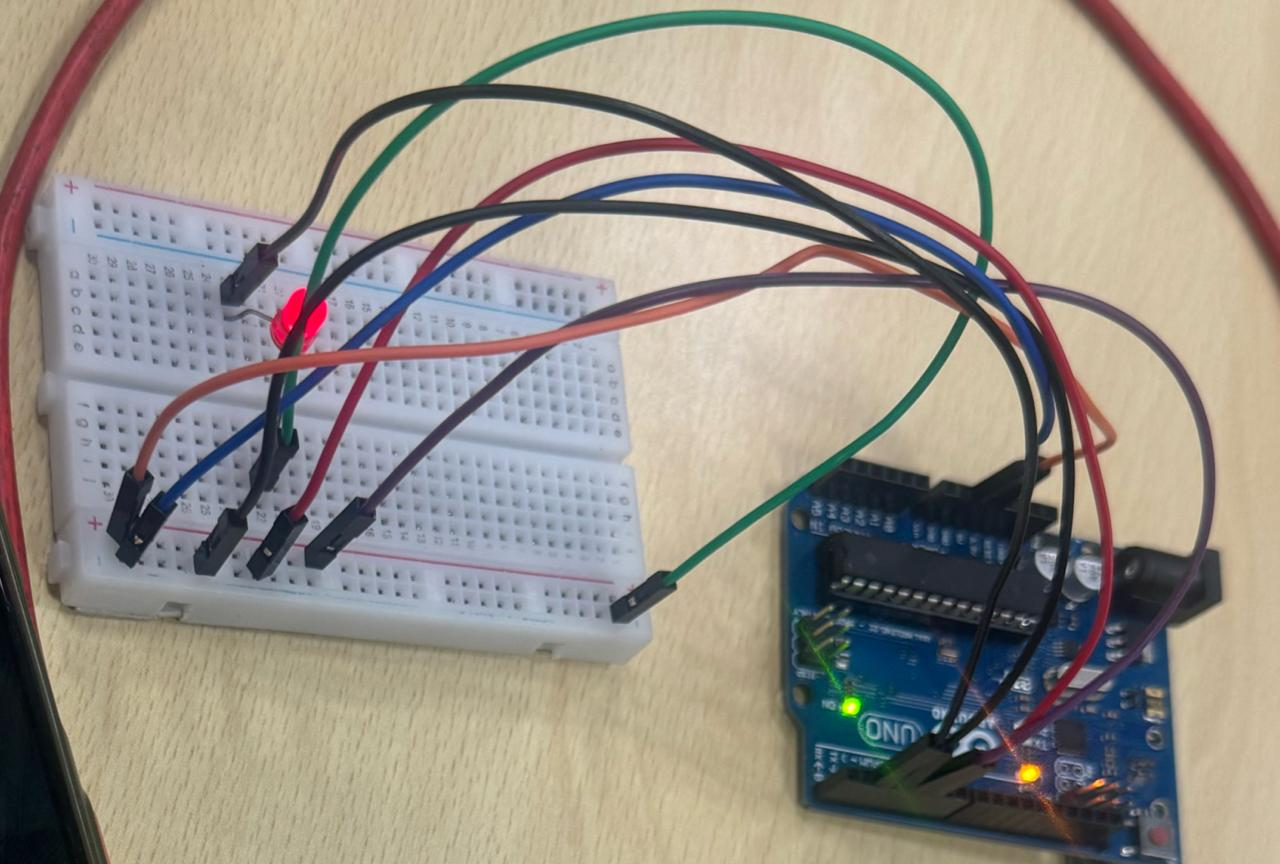
\includegraphics[width=0.4\textwidth]{IMG-20241022-WA0001.jpg}
 \caption{\label{fig:1}}    
\end{figure}
\begin{figure}[h] 
 \centering 
 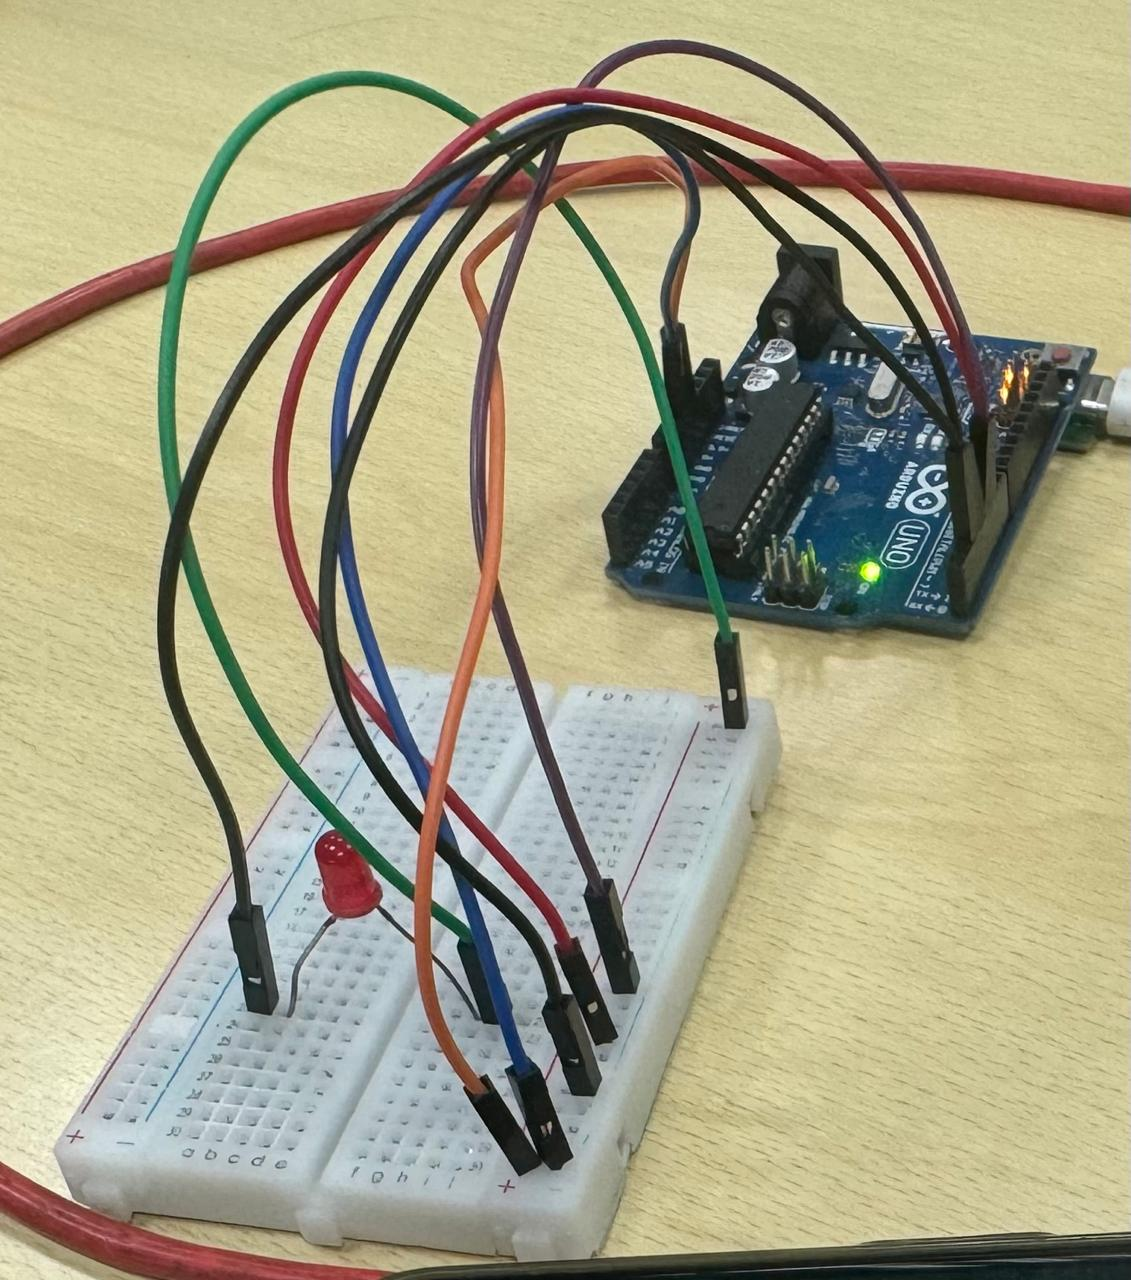
\includegraphics[width=0.4\textwidth]{IMG-20241022-WA0002}
 \caption{\label{fig:2}}    
\end{figure}
\section{CONCLUSION}
The experiment demonstrates the successful implementation of the simplified Boolean function using an Arduino. The LED’s behavior confirms the accuracy of the function's simplification, as it responds according to the specified truth table when the inputs are adjusted, verifying the logical operation and its hardware execution.
\end{document}
